\documentclass[12pt]{article}


\usepackage[T1]{fontenc}	%better font encoding
\usepackage[utf8]{inputenc}	%better font encoding
\usepackage{graphicx}		%allow insertion of images
\usepackage[usenames,dvipsnames,svgnames,table]{xcolor}		%allow colour
\usepackage{amsmath,amssymb,amsthm,textcomp, xfrac}			%math symbols, etc
\usepackage{enumerate}		
\usepackage{multicol}		%allow multi columns
\usepackage{tikz}			%vector graphics
\usepackage{pgfplots}		%plots in vector graphics
\usepackage{epstopdf}		%eps files
\pgfplotsset{compat=1.8}
\usepackage{nth}
\usepackage{gensymb}
\usepackage{framed}


\usepackage[title,toc,page]{appendix}
\noappendicestocpagenum



% refs
%\usepackage[sorting=none]{biblatex}
%\usepackage[utf8]{inputenc}
%\usepackage{csquotes}
%\bibliography{ENGR_297}

% to do notes
\usepackage{todonotes}

%tables
\usepackage{booktabs}		%professional tables
\usepackage{tabularx, booktabs}
\newcolumntype{Y}{>{\centering\arraybackslash}X}	%type Y - even column width - centered
\usepackage{multirow}
\usepackage{bigstrut}
\usepackage{diagbox}
%\usepackage{slashbox}

%blank page
\newcommand*\NewPage{\newpage\null\thispagestyle{empty}\newpage}

\usepackage{color}
\usepackage[hidelinks]{hyperref}	%hyperlinks
\hypersetup{
%    colorlinks=false, 	%set true if you want colored links
    linktoc=all,     	%set to all if you want both sections and subsections linked
%    linkcolor=blue,  	%choose some color if you want links to stand out
}

%sideways figures
\usepackage{rotating}
\usepackage{pdflscape} %pdflscap for electronic  lscap for print
\usepackage{capt-of}

\usepackage{adjustbox}
\usepackage{blindtext}


%units
\usepackage{siunitx}
\usepackage{cancel}
\sisetup{load-configurations = abbreviations}
\sisetup{per-mode = fraction}
%\sisetup{per-mode = symbol}

%%section style
%\usepackage{titlesec}
%\titleformat{\section}[runin]
%{\normalfont\bfseries}
%{\thesection.}{.5em}{}[]
%
%\titleformat{\subsection}[runin]
%{\normalfont\bfseries}
%{\thesubsection}{.5em}{}[]
%\setcounter{secnumdepth}{0} %dont number sections

%disable indents
%\usepackage{parskip}

%chemistry
\usepackage[version=3]{mhchem}

%scientific notation  use \e
\providecommand{\e}[1]{\ensuremath{\times 10^{#1}}}

%diferential
\def \d {\ensuremath{\mathrm{d}}}

%email
\newcommand{\email}[1]{\href{mailto:#1}{\texttt{#1}}}


%uppercase subscripts
\usepackage{relsize}
\newcommand{\s}[1]{_{\!\mathsmaller{#1}}}

\usepackage{fullpage}		%set full page margins

\newcommand{\linia}{\rule{\linewidth}{0.5pt}}

\usepackage{pdfpages}
% custom footers and headers
\usepackage{lastpage}
\usepackage{fancyhdr}
\pagestyle{fancy}
\lhead{}
\chead{}
\rhead{}
\lfoot{}
\cfoot{\thepage}
\rfoot{}
\renewcommand{\headrulewidth}{0pt}
\renewcommand{\footrulewidth}{0pt}
%

\begin{document}

\begin{titlepage}
\newcommand{\HRule}{\rule{\linewidth}{0.5mm}} 
\center 

% Title Page Headings
\textsc{\LARGE University of Victoria}\\[0.25cm]
\textsc{\Large Faculty of Engineering}\\[0.5cm]
\textsc{\large TERM YEAR Work Term Report}\\[0.5cm] %date

\HRule \\[0.4cm]
{ \huge \bfseries TITLE}\\ % Document Title
\HRule \\[1 cm]
 
\begin{center}\large
Department of Mechanical Engineering\\
University of Victoria\\
Victoria, BC\\[1cm]

FIRST \textsc{LAST}	\\ %your name
V0011111111	\\
Work Term ?	\\
Mechanical Engineering\\
\email{email@uvic.ca}\\[1cm]
\end{center}


{\large \today}\\[0.5cm] % Date


\includegraphics{UVic_logo}\\[0.5cm]


\noindent\makebox[\textwidth][c]{
\begin{minipage}{1.1\textwidth}
\begin{flushleft}
\begin{framed}
	\textbf{Supervisor's Approval: To be completed by Employer}	\\
	I approve the release of this report to the University of Victoria for evaluation purposes only.\\
	The report is to be considered (select one): $ \square $ NOT CONFIDENTIAL $ \square $ CONFIDENTIAL\\
	\vspace{.25cm}
	Signature: \underline{\hspace{4.3 cm}} Position: \underline{\hspace{4 cm}}  Date: \underline{\hspace{3 cm}} \\
	\vspace{.25cm}
	Name (print): \underline{\hspace{4 cm}} E-Mail: \underline{\hspace{4 cm}} Fax : \underline{\hspace{3 cm}} \\
	If a report is deemed CONFIDENTIAL, a non-disclosure form signed by an evaluator will be faxed to the employer. The report will be destroyed following evaluation. If the report is NOT
	CONFIDENTIAL, it will be returned to the student following evaluation.
\end{framed}
\end{flushleft}
\end{minipage}
}




\end{titlepage}

%\NewPage %blank added for double sided printing



\clearpage



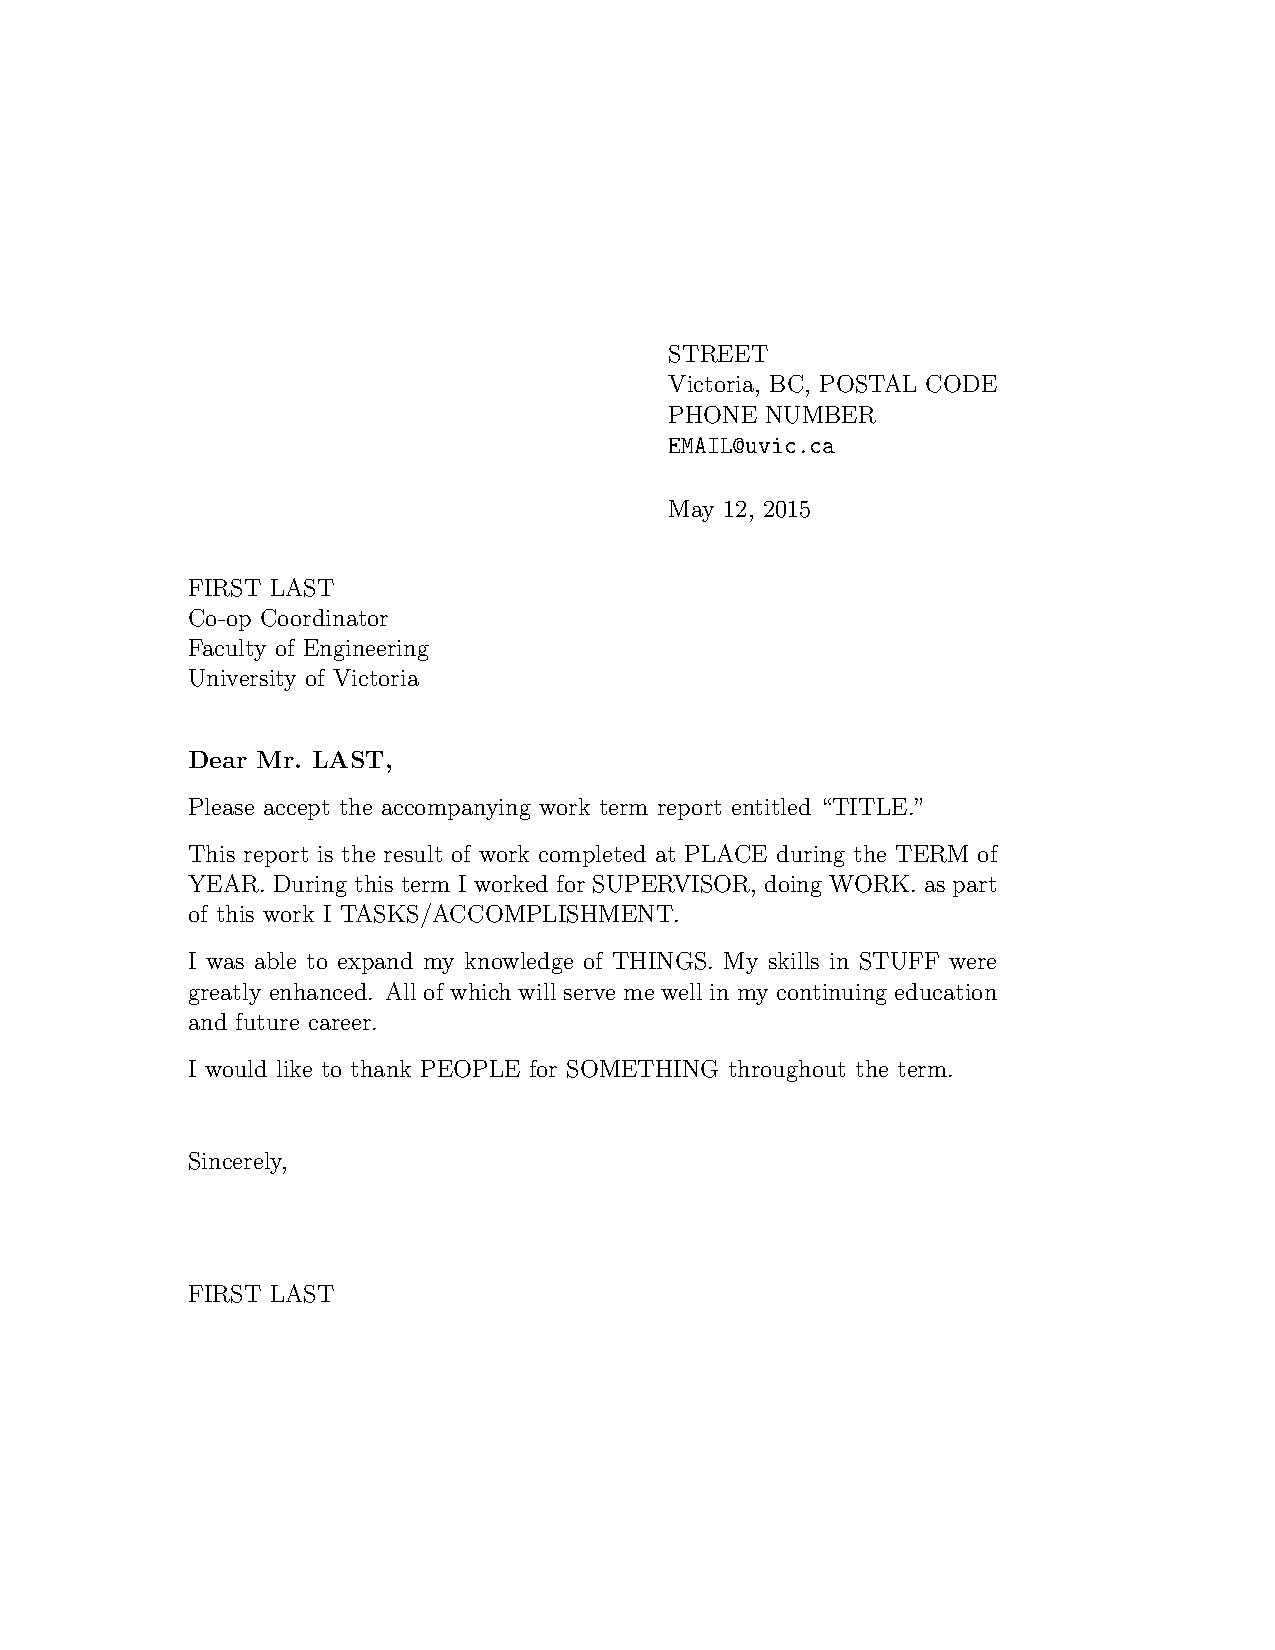
\includepdf[]{./Letter/letter.pdf}




\pagenumbering{roman}
%\setcounter{page}{1}
\tableofcontents



\cleardoublepage
%\phantomsection

\listoffigures \addcontentsline{toc}{section}{\listfigurename}

\pagebreak

\section*{Summary} \addcontentsline{toc}{section}{Summary}

\pagebreak

\section*{Glossary} \addcontentsline{toc}{section}{Glossary}

\newpage
%%%%%%%%%%%%%%%%%%%%%%%%%%%%%%%%%%%%%%%%%%%%%%%
%%%%          Document Starts Here      %%%%%%%



\pagenumbering{arabic}
\section{Introduction}



\section{Discussion}




\section{Conclusions}

\section{Recommendations}


	\begin{table} [h]
		content...
		\caption{tab 1}
	\end{table}

	\begin{figure} [h]
		\caption{fig 1}
	\end{figure}
	
\pagebreak

\begin{appendices}


\addtocontents{toc}{\protect\setcounter{tocdepth}{-1}}
\cfoot{\thesection-\thepage}
\pagenumbering{arabic}

\section{app1 name}

\pagebreak
\section{app2 name}
\pagenumbering{arabic}

\pagebreak
\section{app3 name}

\pagenumbering{arabic}



\pagebreak

\end{appendices}


\end{document}